\section{Robot (Reinforcement) Learning}
\label{sec:learning-rl}

\epigraph{\textit{Approximate the solution, not the problem} [...]}{Richard Sutton}

\begin{tldr}
The need for expensive, high-fidelity simulators can be obviated learning from real-world data, using sample-efficient algorithms that can safely train directly on hardware.
\end{tldr}

\begin{figure}
    \centering
    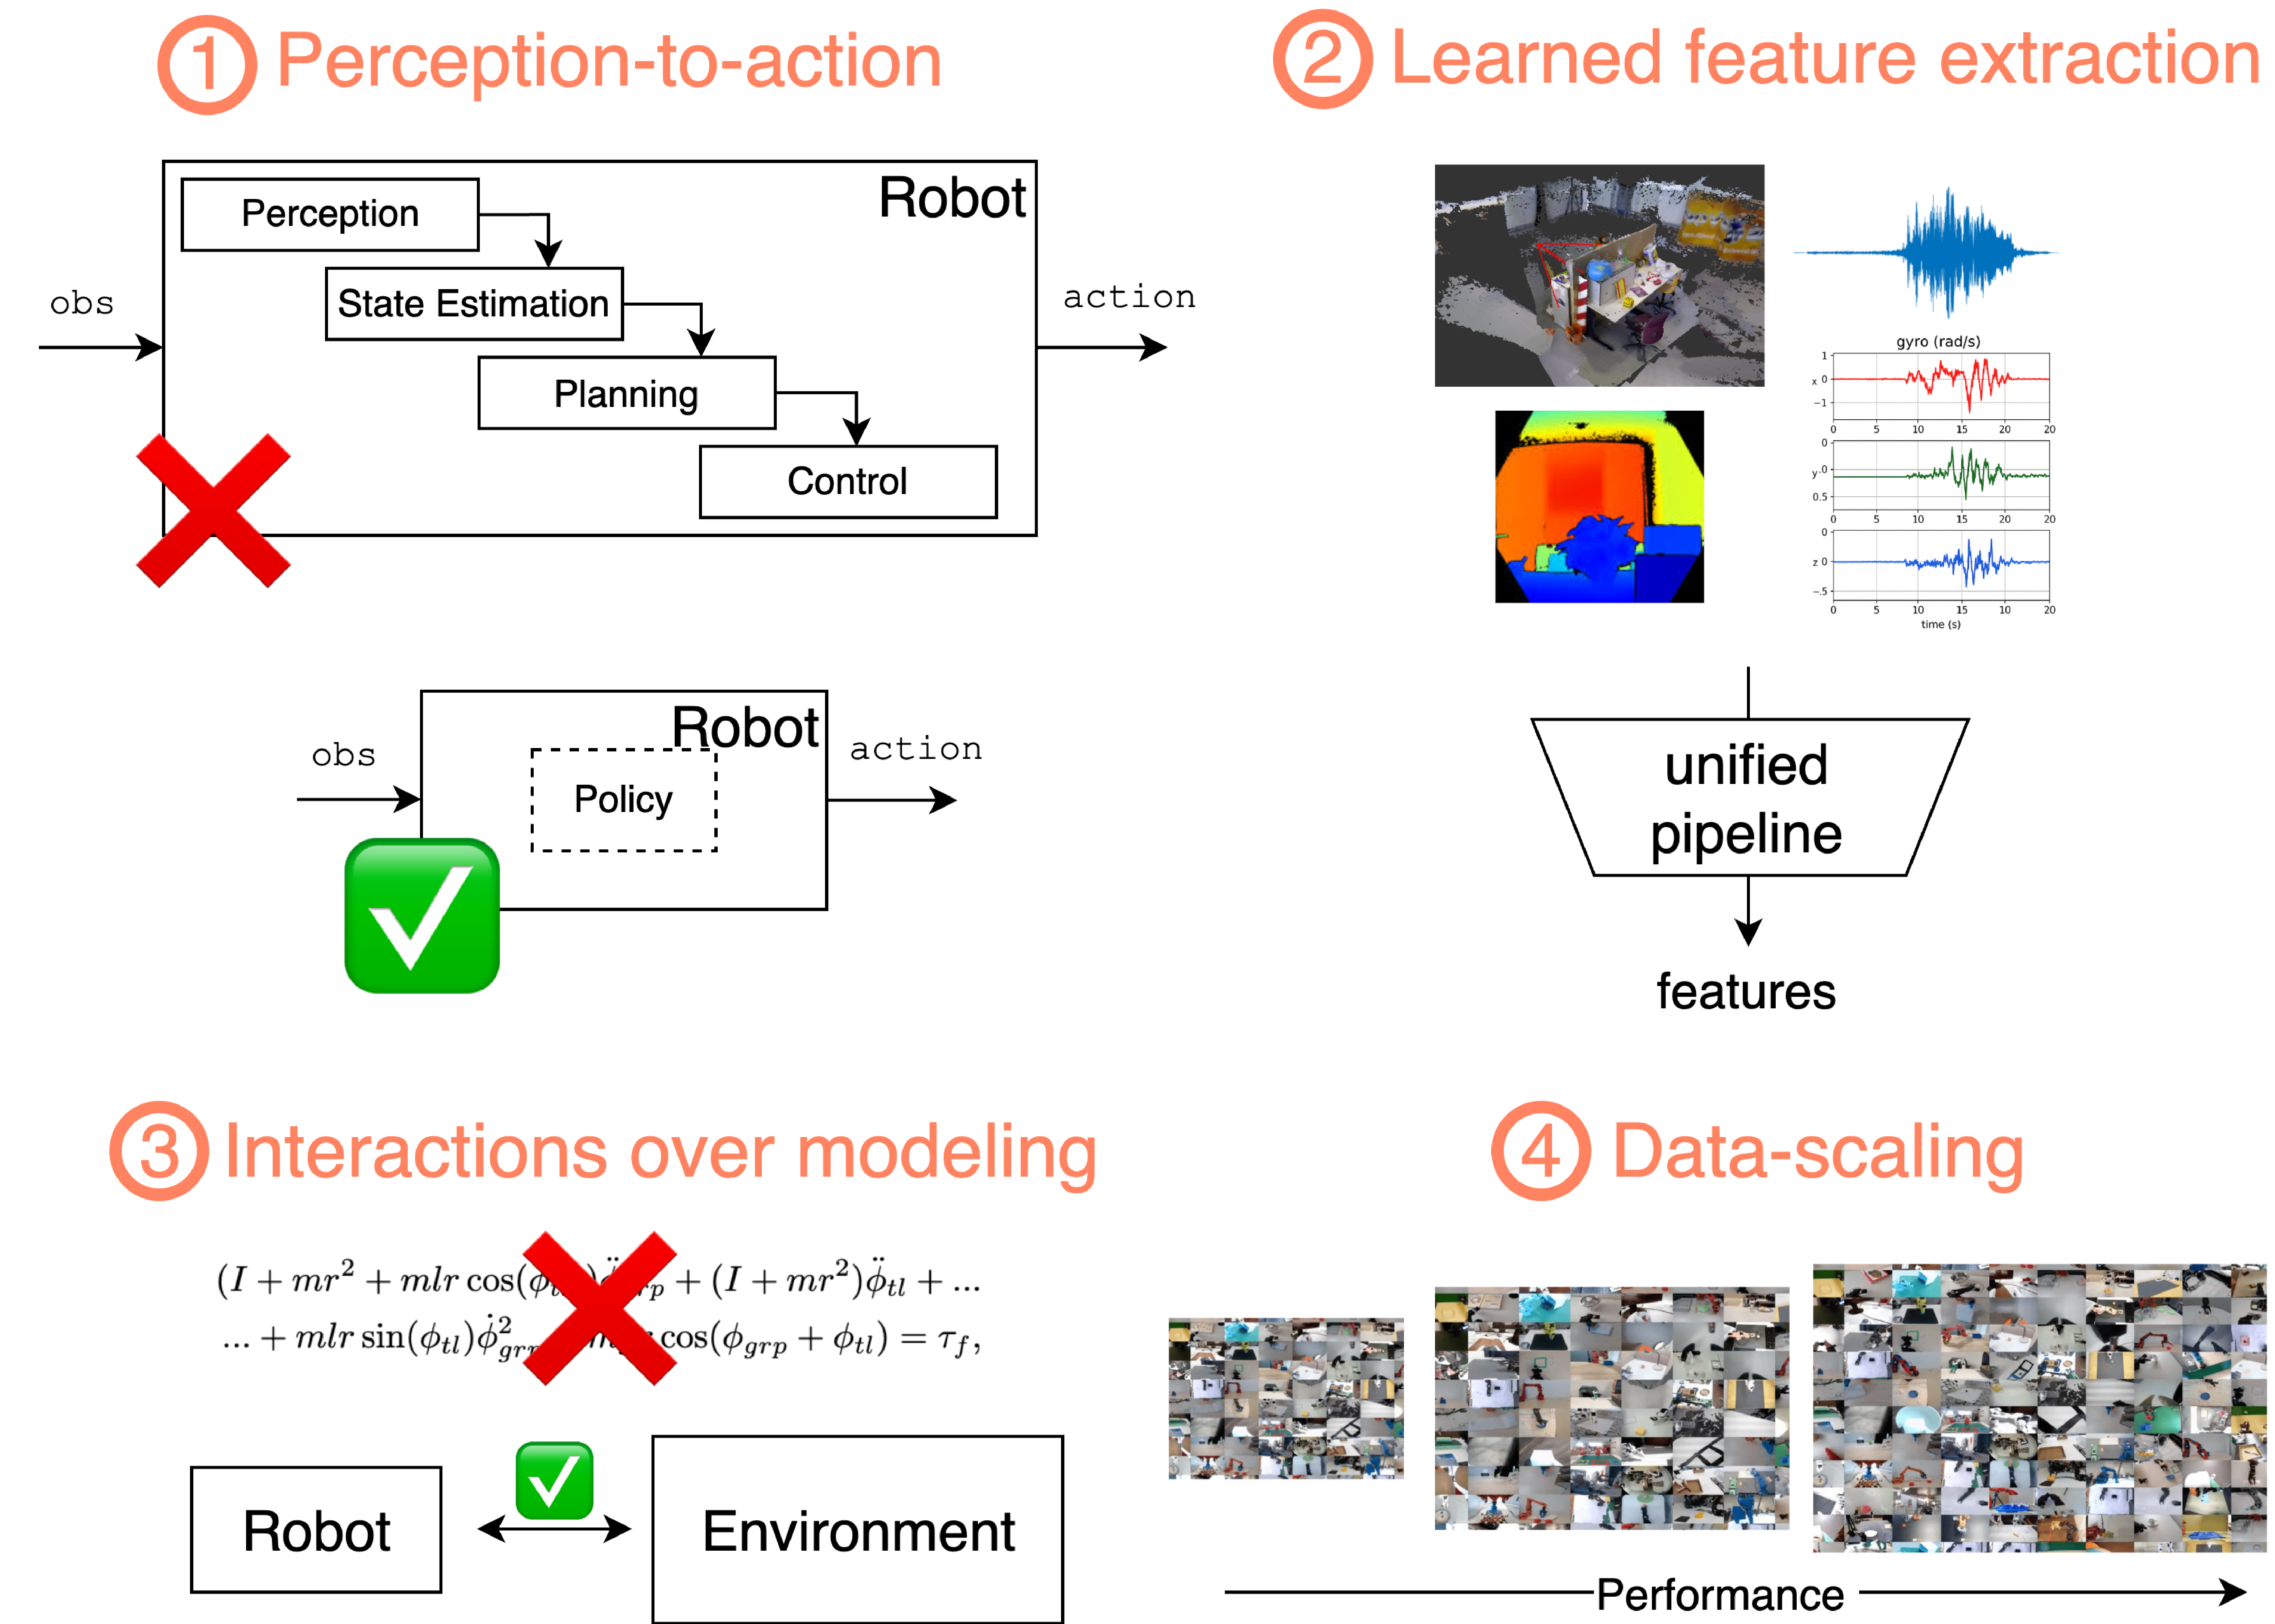
\includegraphics[width=0.9\linewidth]{figures/ch3/ch3-learning-benefits.png}
    \caption{Learning-based robotics streamlines perception-to-action by learning a (1) unified high-level controller capable to take (2) high-dimensional, unstructured sensorimotor information. Learning (3) does not require a dynamics model and instead focuses on interaction data, and (4) empirically correlates with
    the scale of the data used.
    }
    \label{fig:robot-learning-upsides}
\end{figure}

Learning-based techniques for robotics naturally address the limitations presented in Section~\ref{sec:classical} (Figure~\ref{fig:robot-learning-upsides}).
In particular, learning-based techniques typically rely on monolithich prediction-to-action pipelines (\emph{visuomotor policies}) which do directly map sensorimotor inputs to predicted actions, streamlining control policies by removing the need to interface multiple components.
Mapping sensory inputs to actions also makes it possible to incorporate diverse input modalities, leveraging the automatic feature extraction capabilities of modern learning systems. 
Moreover, learning-based approaches can, in principle, bypass explicit modeling altogether and instead rely solely on interaction data---an advantage that proves transformative when dynamics are difficult to model or entirely unknown.
Lastly, learning for robotics (\emph{robot learning}) is naturally well posed to leverage the growing amount of robotics data openly available, just as computer vision and natural language processing did historically benefit from large-scale corpora of data, in great part overlooked by dynamics-based approaches.

Being a field at its relative nascent stages, no prevalent technique(s) proves distinctly better than any other in the domain of robot learning.
Still, two major classes of methods gained prominence: \highlight{Reinforcement Learning (RL)} and \highlight{Behavioral Cloning (BC)} (Figure~\ref{fig:robot-learning-atlas}).
In this section, we provide a conceptual overview of applications of RL to robotics, as well as introduce practical examples of how to use RL within \lerobot.
We then introduce the major limitations RL suffers from, to introduce BC techniques in Section~\ref{sec:learning-bc-single} and Section~{sec:learning-foundation}.

\begin{wrapfigure}[23]{r}{0.3\textwidth}
    \vspace{-\intextsep}
    \centering
    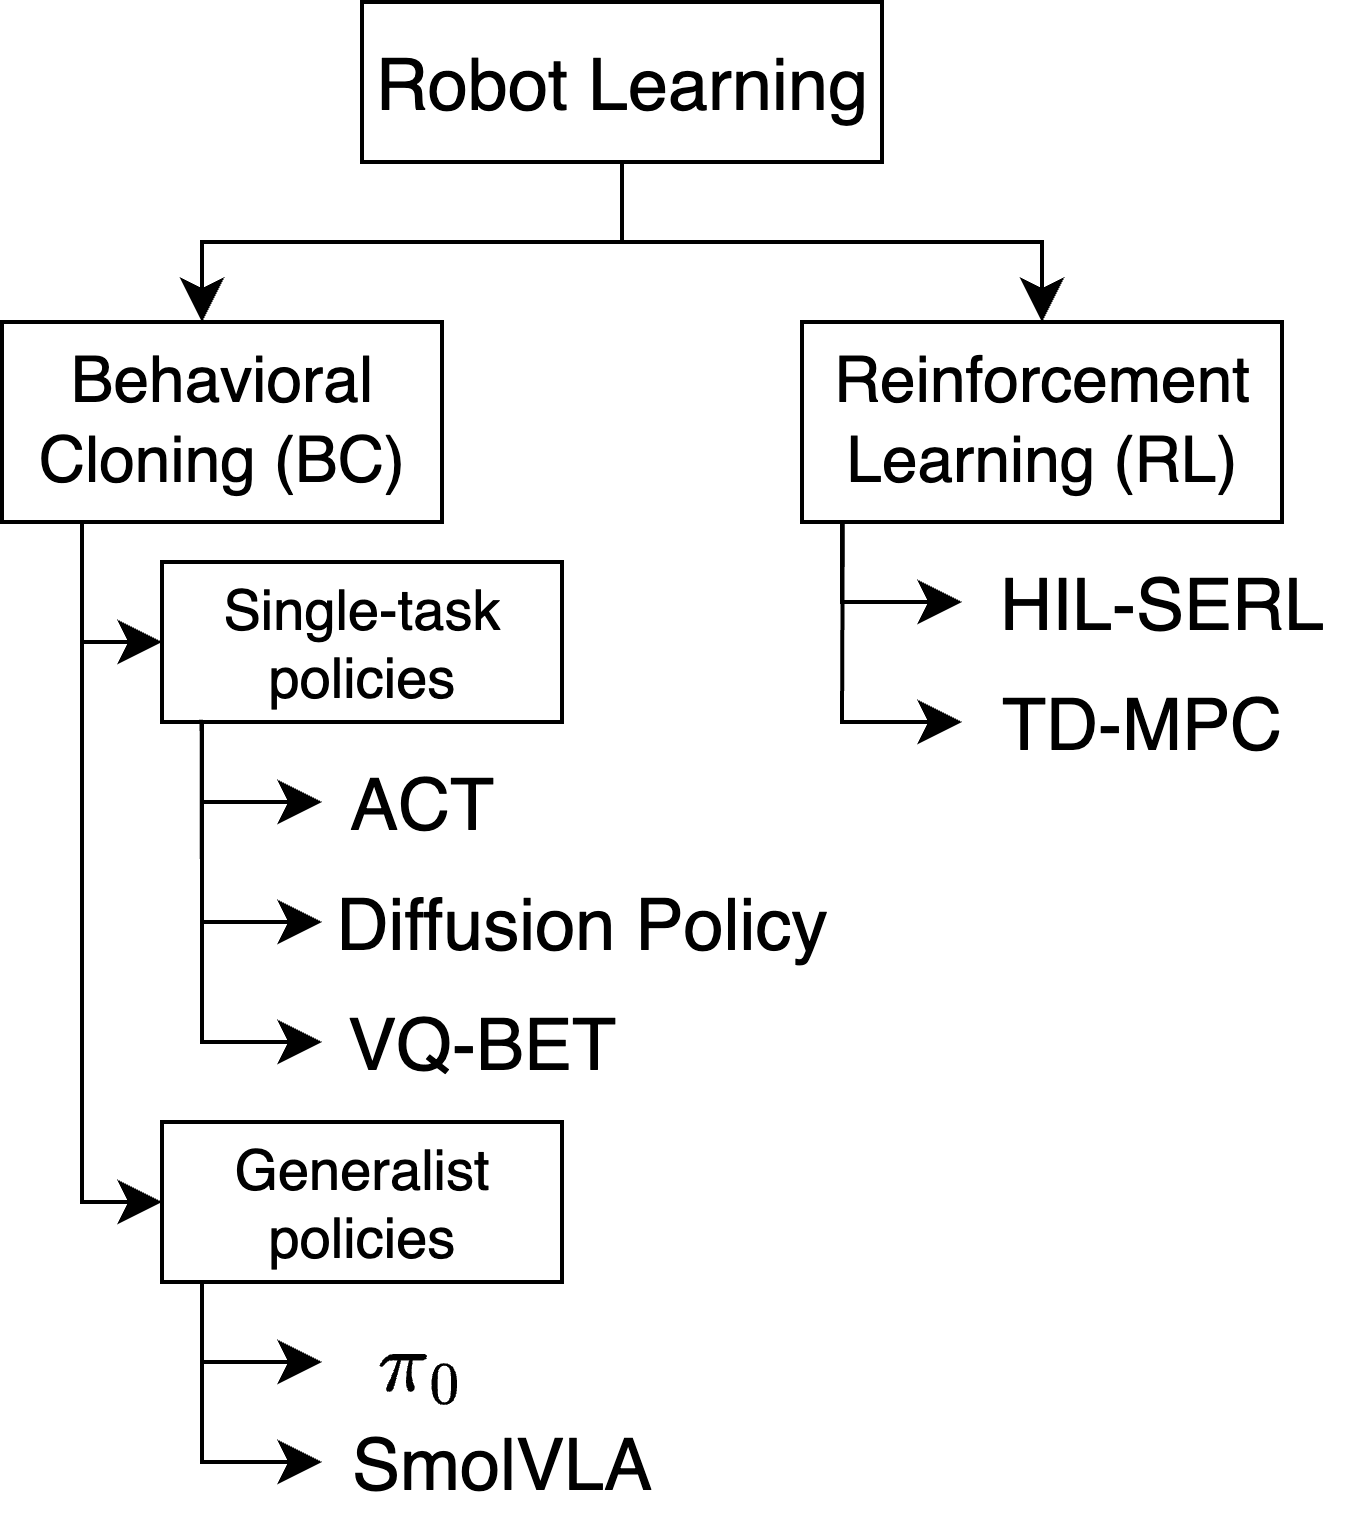
\includegraphics[width=\linewidth]{figures/ch3/ch3-learning-atlas.png}
    \caption{Overview of the robot learning methods implemented in \lerobot. All algorithms are implemented in Pytorch. References:~\citet{zhaoLearningFineGrainedBimanual2023,chiDiffusionPolicyVisuomotor2024,leeBehaviorGenerationLatent2024,black$p_0$VisionLanguageActionFlow2024,shukorSmolVLAVisionLanguageActionModel2025,luoPreciseDexterousRobotic2024,hansenTemporalDifferenceLearning2022} (top-to-bottom, left-to-right).}
    \label{fig:robot-learning-atlas}
\end{wrapfigure}

In Figure~\ref{fig:robot-learning-atlas} we deliberately include generalist robot models~\citep{black$p_0$VisionLanguageActionFlow2024,shukorSmolVLAVisionLanguageActionModel2025} alongside task-specific BC methods.
While significantly different in spirit---\emph{generalist} models are language-conditioned and use instructions to generate motion valid across many tasks, while \emph{task-specific} models are typically not language-conditioned and used to perform a single task---\emph{foundation} models are still largely trained to reproduce trajectories contained in a (large) training set of input demonstrations.
Thus, we argue generalist policies can indeed be grouped alongside other task-specific BC methods, as they both leverage similar training data and schemas.
Figure~\ref{fig:robot-learning-atlas} illustrates this categorization graphically, explicitly listing all the robot learning policies currently available in \lerobot: Action Chunking with Transformers (ACT)~\citep{zhaoLearningFineGrainedBimanual2023}, Diffusion Policy~\citep{chiDiffusionPolicyVisuomotor2024}, Vector-Quantized Behavior Transformer (VQ-BeT)~\citep{leeBehaviorGenerationLatent2024}, \( \pi_0 \)~\citep{black$p_0$VisionLanguageActionFlow2024}, SmolVLA~\citep{shukorSmolVLAVisionLanguageActionModel2025}, Human-in-the-loop Sample-efficient RL (HIL-SERL)~\citep{luoPreciseDexterousRobotic2024} and TD-MPC~\citep{hansenTemporalDifferenceLearning2022}.


\begin{figure}
    \centering
    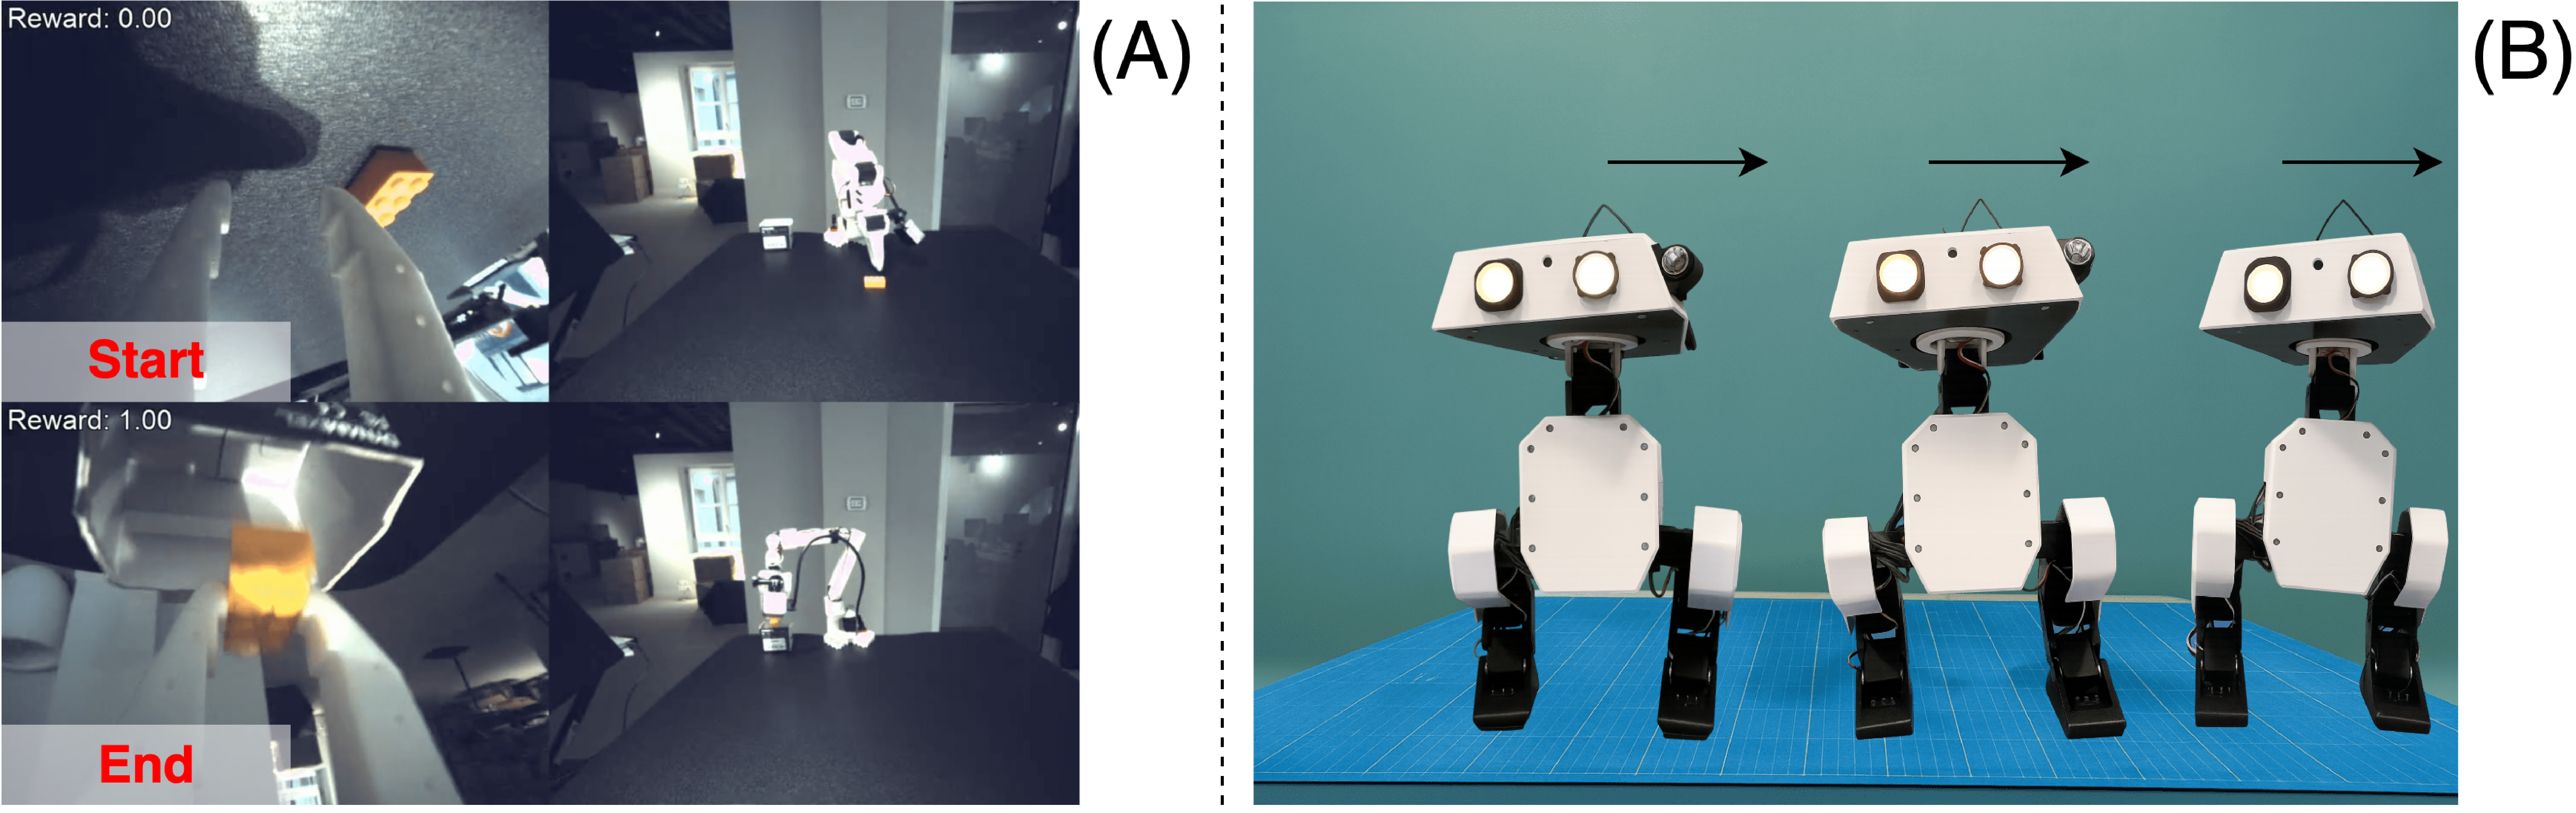
\includegraphics[width=0.8\linewidth]{figures/ch3/ch3-rl-examples.png}
    \caption{Examples of two different robotics tasks performed using RL. In the manipulation task (A) an agent learns to reach for a yellow plastic block in its environment, and to put it inside of a box. In the locomotion task (B) an agent learns to move its center of mass sideways without falling.}
    \label{fig:robotics-with-rl-examples}
\end{figure}

Applications of RL to robotics have been studied long enough that the relationship between these two disciplines has been compared to that of physics and matematics~\citep{koberReinforcementLearningRobotics}.
Indeed, due to their inherently interactive and sequential nature, robotics control problems can be directly cast as RL problems.
Figure~\ref{fig:robotics-with-rl-examples} presents two of such cases.
Reaching for an object to then move it somewhere else in the scene is a sequential problem where over time the controller needs to adjust the position of the robot arm based on the current configuration and the (possibly varying) position of the object.
Figure~\ref{fig:robotics-with-rl-examples} also shows an example of a locomotion problem, where sequentiality is inherent in the problem formulation: while sliding to the side, the controller needs to keep adjusting to the robot's to avoid failure (falling).

\subsection{A (Concise) Introduction to RL}
The RL framework~\citep{suttonReinforcementLearningIntroduction2018}, which we briefly introduce here, has often been used to tackle robotics problems~\citep{koberReinforcementLearningRobotics}.
RL is a subfield within ML fundamentally concerned with the development of autonomous systems (\emph{agents}) capable to \emph{continuously behave} in an evolving environment, developing (ideally, well-performing) control strategies (\emph{policies}).
Crucially for robotics, RL agents improve through trial and error, bypassing explicit models of the problem dynamics in favor of interaction data.
In RL, this feedback loop between actions and outcomes (Figure~\ref{fig:rl-most-famous-pic}) is established through the agent sensing a scalar quantity (\emph{reward}) measuring how desirable a given \emph{transition} is for the accomplishment of its goal.

\begin{figure}
    \centering
    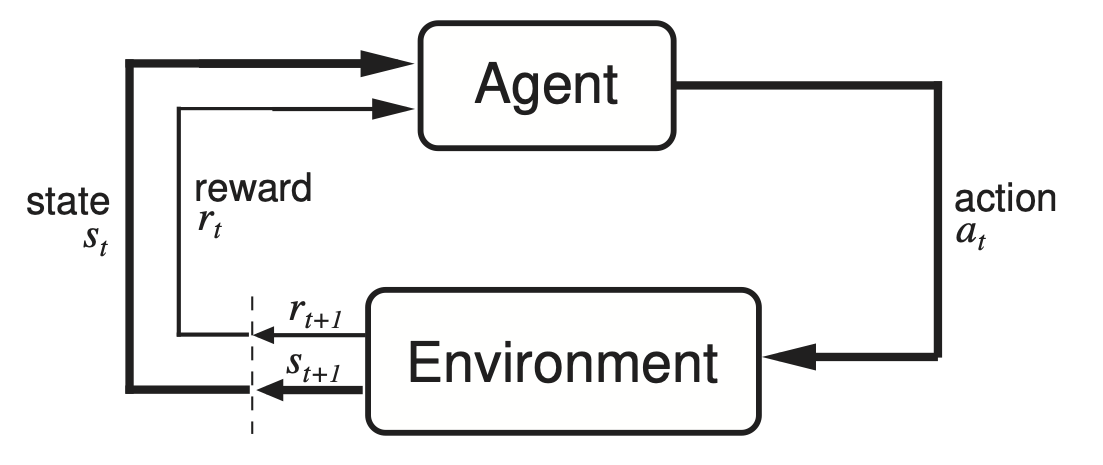
\includegraphics[width=0.5\linewidth]{figures/ch3/ch3-agent-env.png}
    \caption{Agent-Environment interaction diagram (image credits to~\citet{suttonReinforcementLearningIntroduction2018}).}
    \label{fig:rl-most-famous-pic}
\end{figure}

Formally, interactions between an agent and its environment are typically modeled via a Markov Decision Process (MDP)~\citep{bellmanMarkovianDecisionProcess1957}.
Representing robotics problems via MDPs offers several advantages, including (1) incorporating uncertainty through MDP's inherently stochastic formulation and (2) providing a theoretically-sound framework for learning \emph{without} an explicit model of the environment dynamics.
While accommodating a continuous time formulation too, MDPs are typically considered in discrete time in RL, assuming interactions to atomically take place at discrete \emph{timestep} \( t=0,1,2,3, \dots, T \).
MDPs allowing for an unbounded number of interactions (\( T \to + \infty \)) are termed \emph{infinite-horizon}, and opposed to \emph{finite-horizon} MDPs in which \( T \) is finite.
Unless diversely specified, we will only be referring to discrete-time finite-horizon (\emph{episodic}) MDPs.

Formally, a lenght-\(T\) Markov Decision Process (MDP) is a tuple \( \mathcal M = \langle \statespace, \actionspace, \dynamics, r, \gamma, \rho, T \rangle \), where:
\begin{itemize}
    \item \(\statespace\) is the \emph{state space}; \(\state \in \statespace\) denotes the (possibly non-directly observable) environment state at time \(t\). In robotics, states often comprise robot configuration and velocities (\(q_t, \dot q_t\)), and can also accomodate sensor readings such as camera or audio streams.
    %
    \item \(\actionspace\) is the \emph{action space}; \(\action \in \actionspace\) may represent joint torques, joint velocities, or even end-effector commands at timestep \( t \). In general, actions correspond to commands intervenings on the configuration of the robot. 
    %
    \item \(\dynamics\) represents the (possibly non-deterministic) environment dynamics, with \(\dynamics: \statespace \times \actionspace \times \statespace \mapsto [0, 1] \), \( \dynamics \, \transition = \transitionprob \). For instance, for a planar manipulator dynamics could be considered deterministic when the environment is fully described (Figure~\ref{fig:planar-manipulation-simple}), and stochastic when unmodeled disturbances depending on non-observable parameters intervene (Figure~\ref{fig:planar-manipulator-box-velocity}).
    %
    \item \(r: \statespace \times \actionspace \times \statespace \to \mathbb R\) is the \emph{reward function}, weighing the transition \( \transition \) in the context of the achievement of an arbitrary goal. For instance, a simple reward function for quickly moving along the \( x \) axis (Figure~\ref{fig:robotics-with-rl-examples}) could be based on the absolute position of the robot along the \( x \) axis~(\(p_{x_t}\)), present negative penalties for falling over (measured from \( p_{z_t} \)) and a introduce bonuses \( \dot p_{x_t} \) for speed, \(r \transition \equiv r(\state) = p_{x_t} \cdot \dot p_{x_t} - \tfrac{1}{p_{z_t}} \).
\end{itemize}
Lastly, \(\gamma \in [0,1) \) represent the discount factor regulating preference for immediate versus long-term reward (with an effective horizon equal to \( \tfrac{1}{1-\gamma} \)), and \( \rho \) is the distribution over \(\statespace \) for the MDP's \emph{initial}, \( s_0 \sim \rho \).

Therefore, a length-\(T\) \emph{trajectory} is the (random) sequence
\begin{equation}\label{eq:trajectory_definition}
    \tau = \trajectory,
\end{equation}
with per-step rewards defined as \(r_t = r \transition \) for ease of notation.
Interestingly, assuming both the environment dynamics and conditional distribution over actions given states---i.e., the \emph{policy}---to be \emph{Markovian}:
%
\begin{align}
\mathbb P(\stateplusone \vert s_t, a_t, s_{t-1}, a_{t-1}, \dots s_0, a_0 ) &= \mathbb P \transitiongiven \label{eq:dynamics_markovian} \\
\mathbb P(\action \vert \state, a_{t-1}, s_{t-1}, s_0, a_0) &= \mathbb P(\action \vert \state), \label{eq:policy_markovian}
\end{align}
%
the probability of observing a given trajectory \( \tau \) factorizes into:
\begin{equation}\label{eq:traj_prob}
    \mathbb P(\tau) = \mathbb P (s_0) \prod_{t=0}^{T-1} \mathbb P \transitiongiven \ \mathbb P(\action \vert \state).
\end{equation}

Policies \( \mathbb P(\action \vert \state) \) are typically indicated as \( \pi(\action \vert \state) \), often parametrized via \( \theta \), yielding \( \pi_\theta (\action \vert \state )\), and are traine by optimizing the (discounted) \emph{return} associated to a given \( \tau \), i.e. the (random) sum of measured rewards over an arbitrary trajectory, 
\[
    G(\tau) = \sum_{t=0}^{T-1} \gamma^{t} r_t.
\]
In that, agents seek to learn control strategies (\emph{policies}, \( \pi_\theta \)) maximizing the expected return \( \mathbb E_{\tau \sim \pi_\theta} G(\tau) \). 
For a given dynamics \( \mathcal D \)---i.e., for a given problem---taking the expectation over the (possibly random) trajectories resulting from acting according to a certain policy provides a direct, goal-conditioned ordering in the space of all the possible policies \( \Pi \), yielding the (maximization) target \( J : \Pi \mapsto \mathbb R \)
\begin{align}
    J(\pi_\theta) &= \mathbb E_{\tau \sim \mathbb P_{\theta; \mathcal D}} \left[ G(\tau) \right], \label{eq:RL-j-function} \\
    \mathbb P_{\theta; \mathcal D} (\tau) &= \rho \prod_{t=0}^{T-1} \mathcal D \transition \ \pi_\theta (\action \vert \state).\label{eq:traj-probabilities-for-policies}
\end{align}

Crucially, in the RL framework the agent is assumed to only \emph{observe} the environment dynamics and not to intervene on them, and thus eq.~\ref{eq:RL-j-function} varies exclusively with the policy followed.
In turn, MDPs naturally provide a framework to optimize over the space of the possible behaviors an agent might enact (\( \pi \in \Pi \)), searching for the \emph{optimal policy} \( \pi^* = \arg \max_{\theta} J(\pi_\theta) \), where \( \theta \) is the parametrization adopted by the policy set \( \Pi: \pi_\theta \in \Pi, \ \forall \theta \).
Besides providing a target for policy search, \( G(\tau) \) can also be used to discriminate between states \( s_t \) and \(\state, \action\) pairs.
Given any state \( s \in \statespace \)---e.g., given a configuration \( q \) of a robot---the \emph{state-value} function
\[
    V_\pi(s) = \mathbb E_{\tau \sim \pi} \left[ G(\tau) \big \vert s_0 = s \right]
\]
can be used to discriminate between desirable and undesirable state in terms of long-term (discounted) reward maximization, under a given policy \(\pi\).
Similarily, the \emph{state-action} value function also conditions the cumulative discounted reward on selecting action \( a \) when in \( s \), and thereafter act according to \( \pi \),
\[
    Q_\pi(s,a) = \mathbb E_{\tau \sim \pi} \left[ G (\tau) \big \vert s_0 = s, a_0=a \right].
\]
Importantly, value functions are interrelated:
\begin{align}
Q_\pi(s_t, a_t) &= \mathbb{E}_{\stateplusone \sim \mathbb P(\bullet \vert \state, \action)} \left[ r_t + \gamma V_\pi(\stateplusone) \right] \label{eq:q-as-v} \\
V_\pi(\state) &= \mathbb E_{\action \sim \pi(\bullet \vert \state)} \left[ Q_\pi (\state, \action) \right],
\label{eq:v-as-q}
\end{align}
inducing an ordering over states and state-action pairs under \( \pi \), and value functions are thus central to most RL algorithms.
A variety of algorithms have been developed in RL attempting to find (approximate) solutions to the problem of maximizing cumulative reward (we report some in Figure~\ref{fig:rl-algos-atlas}).

\begin{figure}
    \centering
    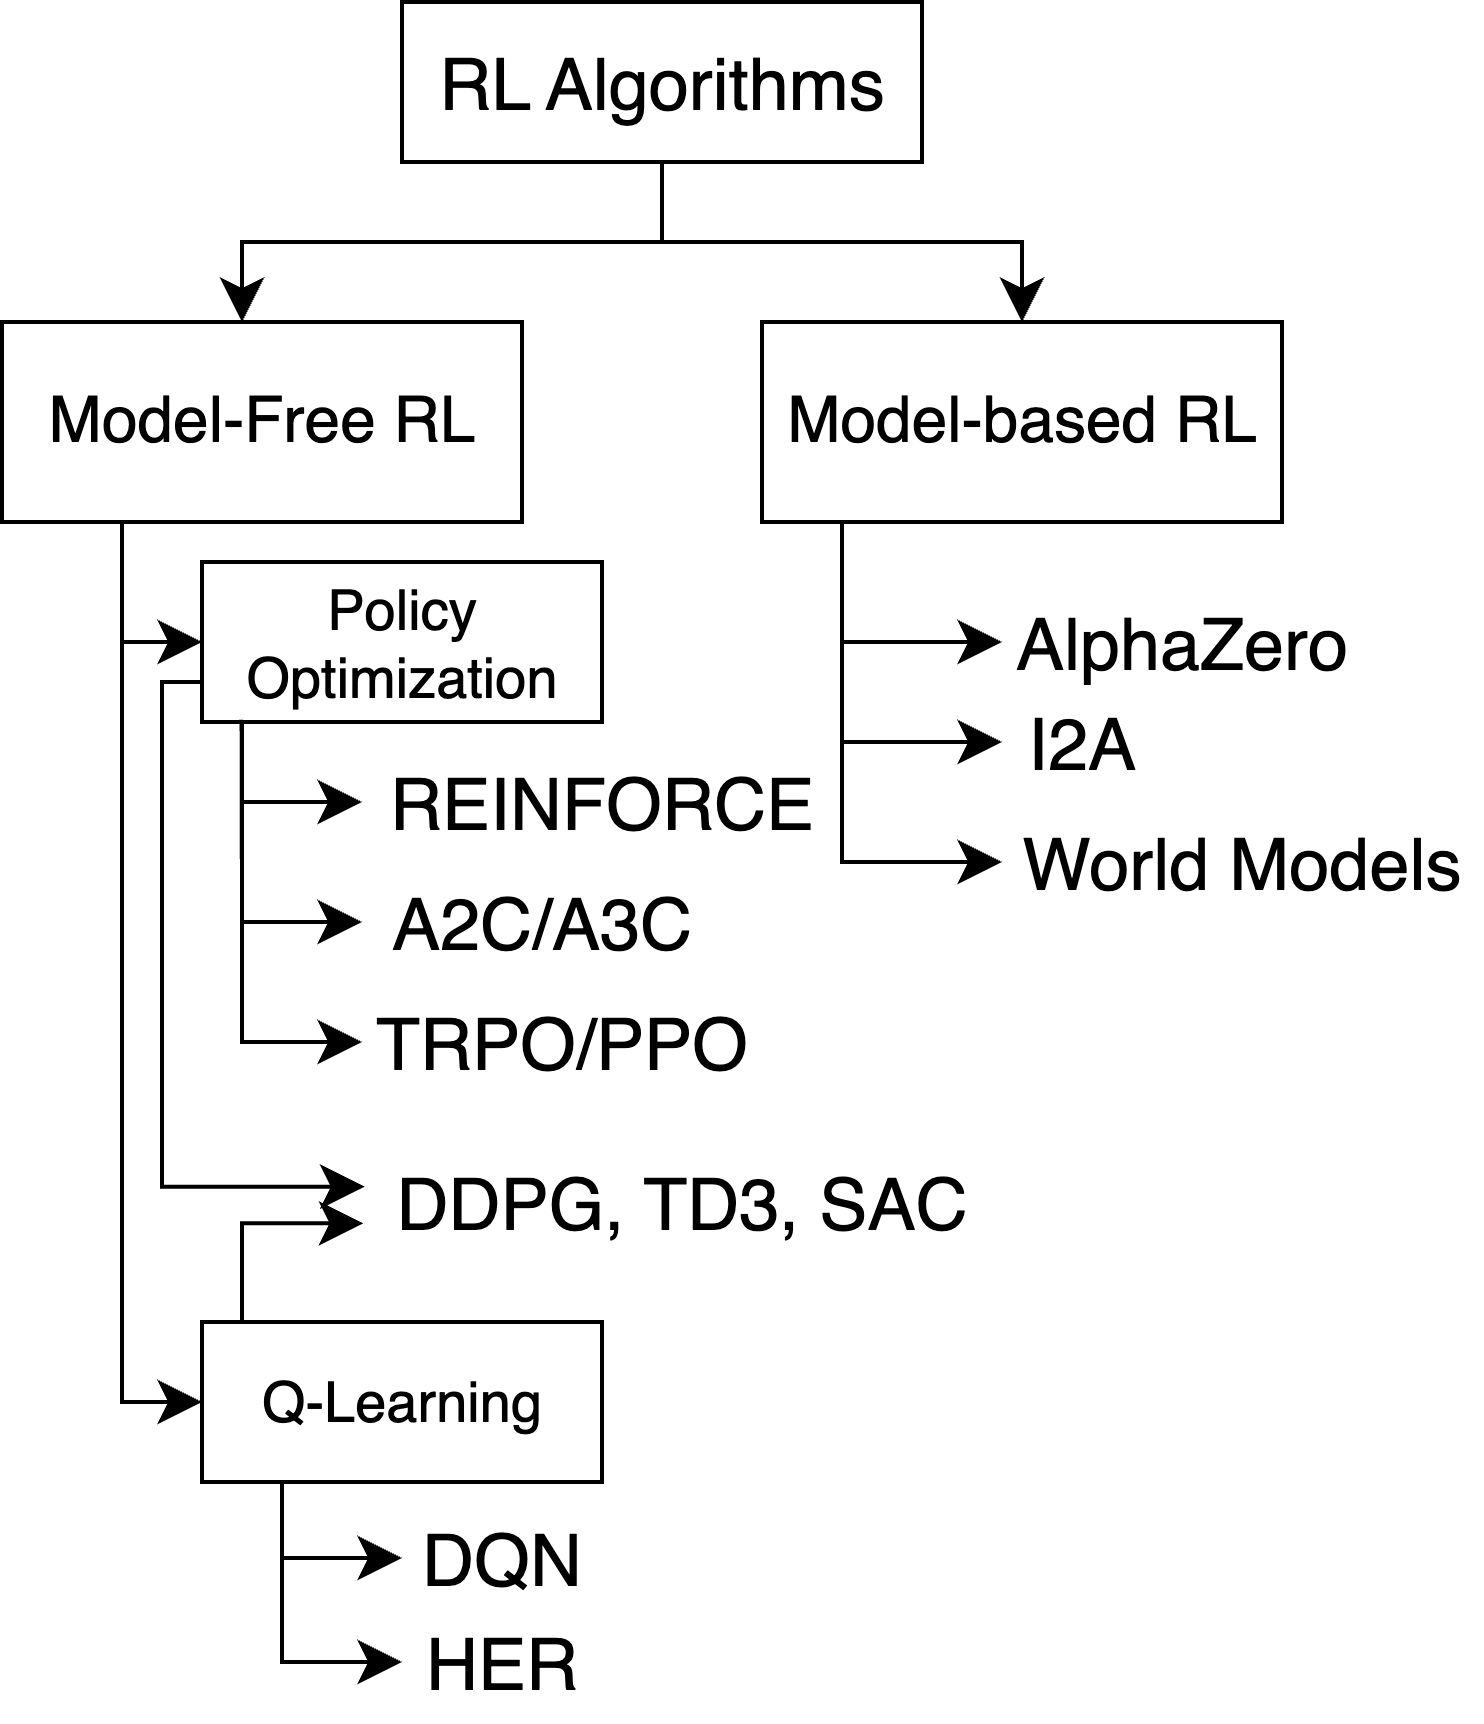
\includegraphics[width=0.4\textwidth]{figures/ch3/ch3-rl-algorithms-atlas.png}
    \caption{Popular RL algorithms. See~\citet{SpinningUp2018} for a complete list of citations.}
    \label{fig:rl-algos-atlas}
\end{figure}

Popular approaches to continuous state and action space---such as those studied within robotics---include~\citet[TRPO]{schulmanTrustRegionPolicy2017},~\citet[PPO]{ schulmanProximalPolicyOptimization2017} and~\citet[SAC]{ haarnojaSoftActorCriticOffPolicy2018}.
Across manipulation~\citep{akkayaSolvingRubiksCube2019} and locomotion problems~\citep{leeLearningQuadrupedalLocomotion2020}, RL proved extremely effective in providing a platform to (1) leverage a unified, streamlined perception-to-action pipeline, (2) natively integrate propioperception with multi-modal high-dimensional sensory streams  (3) disregard a description of the environment dynamics, by focusing on observed interaction data rather than modeling, and (4) anchor policies in the experience collected and stored in datasets.
For a more complete survey of applications of RL to robotics, we refer the reader to~\citet{koberReinforcementLearningRobotics,tangDeepReinforcementLearning2024}.

\subsection{Real-world RL for Robotics}
Streamlined end-to-end control pipelines, data-driven feature extraction and a disregard for explicit modeling in favor of interaction data are all features of RL for robotics.
However, RL still suffers from limitations concerning safety and learning efficiency, particularly pressing for real-world robotics applications.

First, especially early in training, \highlight{actions are typically explorative, and thus may be erractic}.
On physical systems, untrained policies may command high velocities, self-collisiding configurations, or torques exceeding joint limits, leading to wear and potential hardware damage.
Mitigating these risks requires external safeguards (e.g., watchdogs, safety monitors, emergency stops), often incuring in a high degree of human supervision.
Further, in the typical episodic setting considered in most robotics problems, experimentation is substantially slowed down by the need to manually reset the environment over the course of training, a time-consuming and error-prone process.
Second, learning efficiently remains problematic in RL, \highlight{limiting the applicability of RL in real-world robotics due to consequently prohibitive timescales of training}.
Even strong algorithms such as SAC~\citep{haarnojaSoftActorCriticOffPolicy2018} typically require a large numbers of transitions \( \{ \sars \}_{t=1}^N \).
On real-world hardware, generating this data is time-consuming.

\begin{figure}
    \centering
    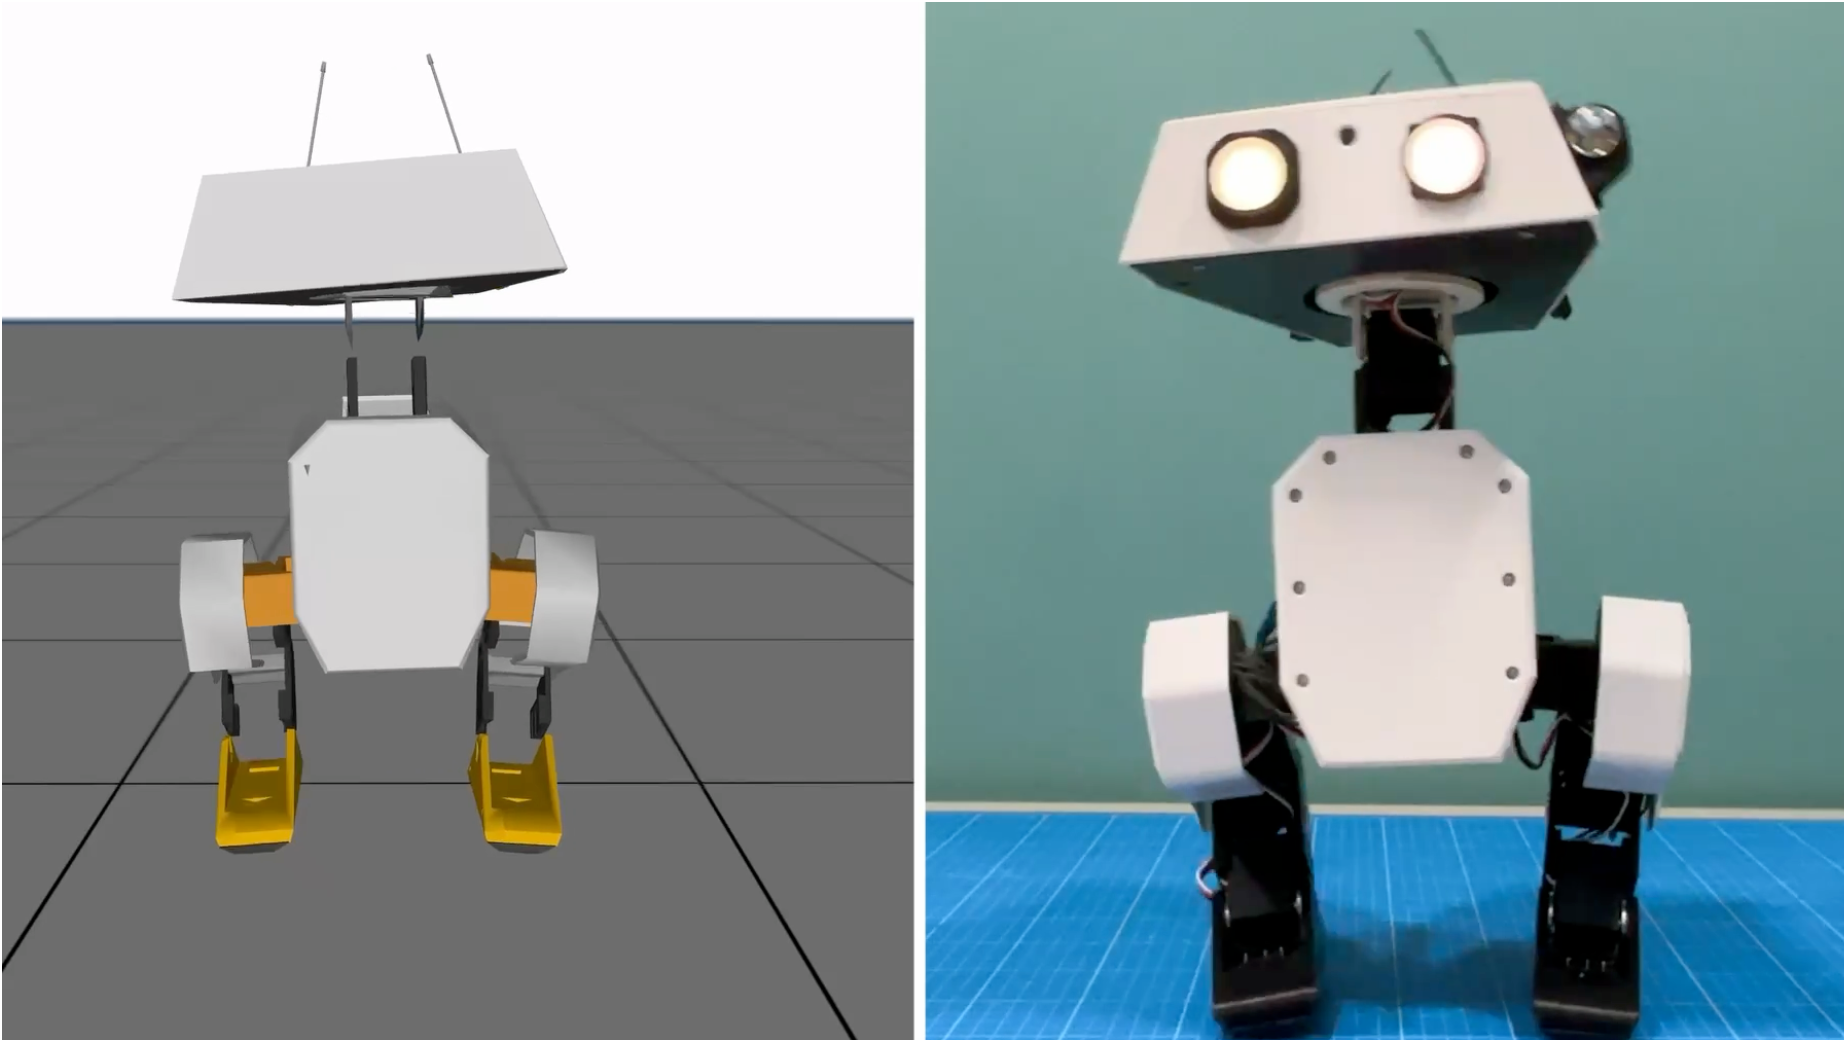
\includegraphics[width=0.7\linewidth]{figures/ch3/ch3-duck-sim-vs-real.png}
    \caption{Simulated (left) vs. real-world (right) OpenDuck. Discrepancies in the simulation dynamics (\emph{reality gap}) pose risks to policy transfer.}
    \label{fig:synthetic-vs-real-duck}
\end{figure}

Training RL policies in simulation~\citep{tobinDomainRandomizationTransferring2017} addresses both issues, eliminating physical risk and dramatically increasing throughput.
Yet, simulators require significant modeling effort, and rely on assumptions (simplified physical modeling, instantaneous actuation, static environmental conditions, etc.) limiting the possibilities to transfer the policies learned in simulation, due the discrepancy between real and simulated environments (\emph{reality gap}, Figure~\ref{fig:synthetic-vs-real-duck}).
\emph{Domain randomization}~\citep{tobinDomainRandomizationTransferring2017} (DR) is a popular technique to overcome the reality gap, and consists in randomizing the parameters of the simulated environment during training, aiming at inducing robustness to specific disturbances.
In this, DR is typically employed to increase the diversity of scenarios over the course of training, improving on the performace sim-to-real transferred policies~\citep{akkayaSolvingRubiksCube2019,antonovaReinforcementLearningPivoting2017,jiDribbleBotDynamicLegged2023}.
In practice, DR is performed training in simulation on simulated dynamics \( \mathcal D \), further parametrized as \( \mathcal D \equiv \mathcal D_\xi \), with a \emph{dynamics} (random) vector \( \xi \) drawn an arbitrary distribution, \( \xi \sim \Xi \).
For instance, one could decide to randomize the friction coefficient of the surface in a locomotion task (Figure~\ref{fig:ducks-on-terrains}), or the center of mass of an object for a manipulation task.
Over the course of training---typically at each episode's reset---a new \( \xi \) is drawn, and used to specify the environment's dynamics for that episode.

\begin{figure}
    \centering
    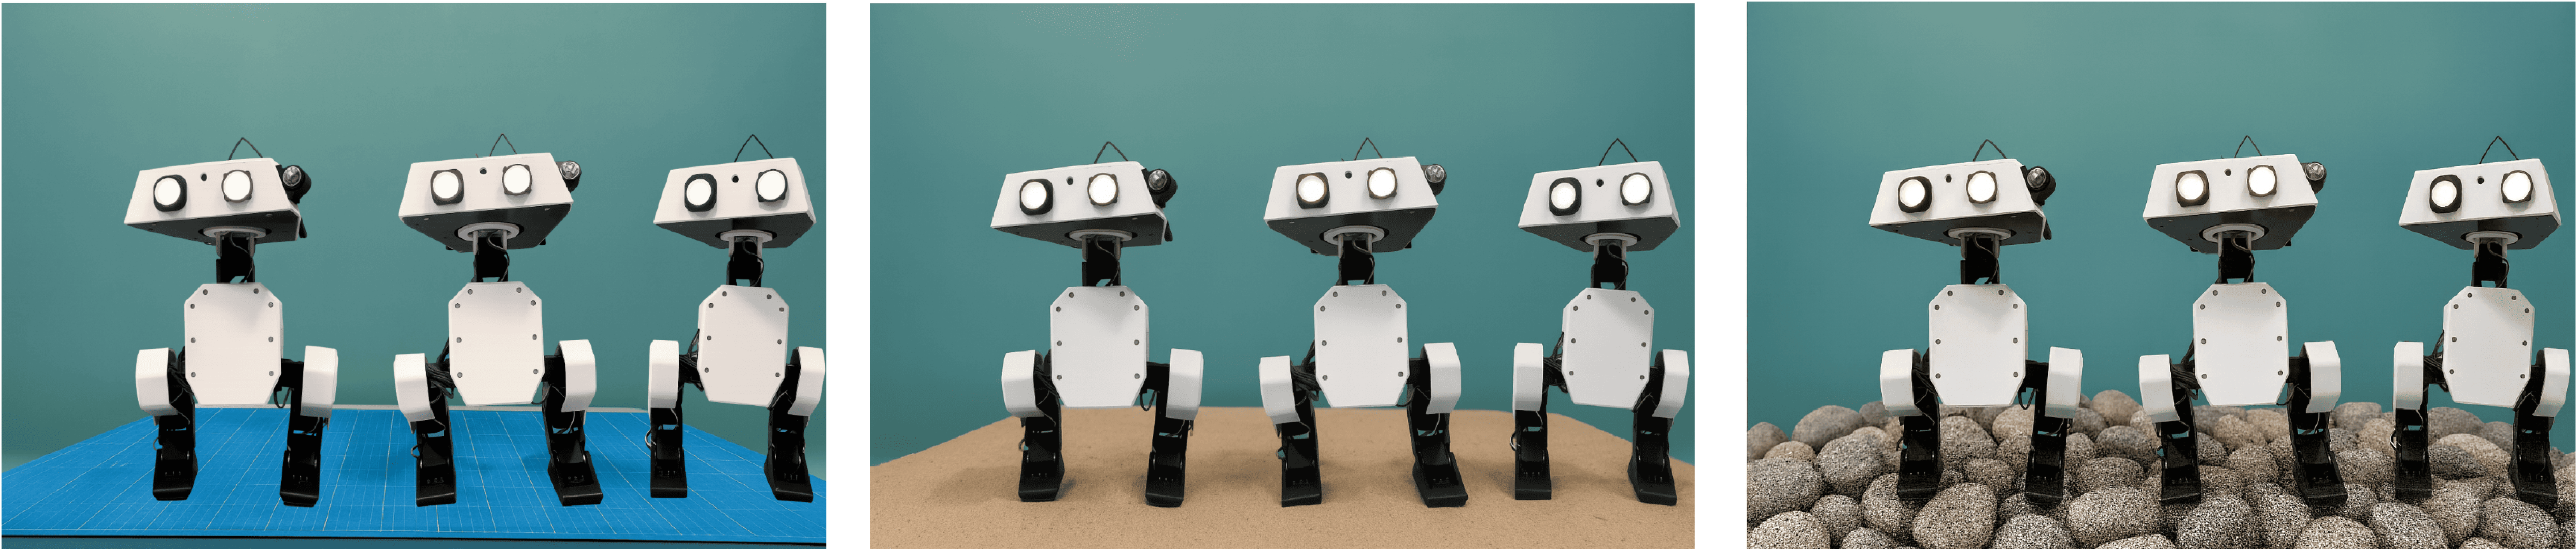
\includegraphics[width=0.9\linewidth]{figures/ch3/ch3-many-ducks.png}
    \caption{The same locomotion task can be carried out in different (simulated) domains (exemplified by the difference in terrains) at training time, resulting to increased robustness over diverse environment dynamics.}
    \label{fig:ducks-on-terrains}
\end{figure}

While effective in transfering policies across the reality gap in real-world robotics~\citep{tobinDomainRandomizationTransferring2017,akkayaSolvingRubiksCube2019, jiDribbleBotDynamicLegged2023,tiboniDomainRandomizationEntropy2024}, DR often requires extensive manual engineering.
First, identifying which parameters to randomize---i.e., the \emph{support} \( \text{supp} (\Xi) \) of \( \Xi \)---is an inherently task specific process.
When locomoting over different terrains, choosing to randomize the friction coefficient is a reasonable choice, yet not completely resolutive as other factors (lightning conditions, external temperature, joints' fatigue, etc.) may prove just as important in practice, making selecting these parameters yet another source of brittlness.

Selecting the dynamics distribution \( \Xi \) is also non-trivial.
On the one hand, distributions with low entropy might risk to cause failure at transfer time, due to the limited robustness induced over the course of training.
On the other hand, excessive randomization may cause over-regularization and hinder performance~\citep{margolisRapidLocomotionReinforcement2022}.
Consequently, the research community investigated approaches to automatically select the randomization distribution \( \Xi \), using signals from the training process or tuning it to reproduce observed real-world trajectories.
\citet{akkayaSolvingRubiksCube2019} use a parametric uniform distribution \( \mathcal U(a, b) \) as \( \Xi \), widening the bounds \( a, b \) as training progresses and the agent's performance improves (AutoDR).
While effective, AutoDR requires significant tuning---the bounds are widened by a fixed, pre-specified amount \( \Delta \) along---and may disregard data when performance \emph{does not} improve after a distribution update~\citep{tiboniDomainRandomizationEntropy2024}. \citet{tiboniDomainRandomizationEntropy2024} propose a similar method to AutoDR (DORAEMON) to evolve \( \Xi \) based on the training signal, but with the key difference of explicitly maximizing the entropy of a parametric Beta distribution---inherently more flexible than uniform distributions---with learned updates instead of fixed \( \Delta \).
In this, DORAEMON proves particularly effective at dynamically increasing the entropy levels of the training distribution by employing an outer-loop max-entropy objective, tackled under performance constraints in the inner-loop RL problem.
Other approaches to automatically perform DR consist in specifically tuning \( \Xi \) to align as much as possible the simulation and real-world domains.
For instance, ~\citet{chebotar2019closing} interleave in-simulation policy training with repeated real-world policy rollouts used to adjust \( \Xi \) based on real-world data, while ~\citet{tiboniDROPOSimtoRealTransfer2023} leverage a single, pre-collected set of real-world trajectories and tune \( \Xi \) under a simple likelihood objective.

While DR has shown promise, it does not address the main limitation that, even under the assumption that an ideal distribution \( \Xi \) was available, many robotics problems \highlight{cannot be simulated with high-enough fidelity under practical computational constraints}.
Simulating contact-rich manipulation of possibly deformable or soft materials---i.e., \emph{folding a piece of clothing}---can prove time-intensive, limiting the benefits of in-simulation training.

A perhaps more foundamental limitation of RL for robotics is the general unavailability of complicated tasks' \emph{dense} reward function, the design of which is essentially based on human expertise, ingenuity and trial-and-error.
In practice, \emph{sparse} reward functions can be used to conclude whether one specific goal has been attained---\emph{has this t-shirt been correctly folded?}---but unfortunately incur in more challenging learning.
As a result, despite notable successes, deploying RL directly on real-world robots at scale remains challenging.

To make the most of (1) the growing number of openly available datasets and (2) relatively inexpensive robots like the SO-100, RL could (1) be anchored in already-collected trajectories---limiting erratic and dangerous exploration---and (2) train in the real-world directly---bypassing the aforementioned issues with low-fidelity simulations.
In such a context, sample-efficient learning is also paramount, as training on the real-world is inherently time-bottlenecked.

Off-policy algorithms like Soft Actor-Critic (SAC)~\citep{haarnojaSoftActorCriticOffPolicy2018} tend to be more sample efficient then their on-policy counterpart~\citep{schulmanProximalPolicyOptimization2017}, due to the presence a \emph{replay buffer} used over the course of training.
Other than allowing to re-use past transitions \( \sars \), the replay buffer can also accomodate for the injection of previously-collected data in the training process~\citep{ballEfficientOnlineReinforcement2023}.
Using expert demonstrations to guide learning together with learned rewards, RL can be effectively carried out in the real-world~\citep{luoSERLSoftwareSuite2025}.
Interestingly, when complemented with in-training human interventions, real-world RL agents have been shown to learn policies with near-perfect success rates on challenging manipulation tasks in 1-2 hours~\citep{luoPreciseDexterousRobotic2024}.

% DQN to DDPG to SAC
\paragraph{Sample-efficient RL}
In an MDP, the optimal policy \( \pi^* \) can be derived from its associated \qfunction, \( Q^* \equiv Q_{\pi^*} \), and in particular the optimal action(s) \(\mu(\state)\) can be selected maximizing the optimal \qfunction \ over the action space,
\[
\mu(\state) = \max_{\action \in \mathcal A} Q^*(\state, \action).
\]
Interestingly, the \qopt-function satisfies a recursive relationship (\emph{Bellman equation}) based on a very natural intuition%
\footnote{Quote from~\citet{mnihPlayingAtariDeep2013}. The notation used has slightly been adapted for consistency with the rest of this tutorial.}:
\begin{quote}
    [...] If the optimal value \( Q^*(\stateplusone, a_{t+1}) \) of the [state] \(\stateplusone \) was known for all possible actions \(a_{t+1} \), then the optimal strategy is to select the action \( a_{t+1}\) maximizing the expected value of \( r_t + \gamma Q^*(s_{t+1}, a_{t+1}) \)
\[ 
Q^*(s_t, a_t) = \mathbb E_{s_{t+1} \sim \mathbb P(\bullet \vert s_t, a_t)} \left[ r_t + \gamma \max_{a_{t+1} \in \mathcal A} Q^*(s_{t+1}, a_{t+1}) \big\vert s_t, a_t  \right]
\]
\end{quote}

In turn, the optimal \qfunction \ %
is guaranteed to be self-consistent by definition.
\emph{Value-iteration} methods exploit this relationship (and/or its state-value counterpart, \( V^*(s_t) \) ) by iteratively updating an initial estimate of \qopt, \( Q_k \) using the Bellman equation as update rule (\emph{Q-learning}):
\[
    Q_{i+1}(s_t, a_t) \leftarrow \mathbb E_{s_{t+1} \sim \mathbb P(\bullet \vert s_t, a_t)} \left[ r_t + \gamma \max_{a_{t+1} \in \mathcal A} Q_i (s_{t+1}, a_{t+1}) \big\vert s_t, a_t  \right],  \quad i=0,1,2,\dots,K
\]
Then, one can derive the (ideally, near-optimal) policy by explicitly maximizing over the action space the final (ideally, near-optimal) estimate \( Q_K \approx Q^* \) at each timestep. 
Indeed, one can show that under certain assumptions on the MDP considered, \( Q_K \to Q^* \, \text{as } K \to \infty \).

Effective in its early applications to small-scale discrete problems, vanilla Q-learning was found complicated to scale to large \( \statespace \times \actionspace \) problems, in which storing \( Q : \statespace \times \actionspace \mapsto \mathbb R \) alone might result prohibitive. 
Also, vanilla Q-learning is not directly usable for \emph{continuous}, unstructured state-action space MPDs, such as those considered in robotics.
In their seminal work on \emph{Deep Q-Learning} (DQN),~\citet{mnihPlayingAtariDeep2013} propose learning Q-values using deep convolutional neural networks, thereby accomodating for large and even unstructured \emph{state} spaces.
DQN parametrizes the Q-function using a neural network with parameters \( \theta \), updating the parameters by sequentially minimizing the expected squared temporal-difference error (TD-error, \( \delta_i \)):
\begin{align}
\mathcal L(\theta_i) &= \mathbb E_{(s_t, a_t) \sim \chi(\bullet)} 
    \big[ 
        (\underbrace{y_i - Q_{\theta_i}(s_t, a_t)}_{\delta_i})^2 
    \big], \label{eq:dqn-loss} \\
    y_i &= \mathbb E_{s_{t+1} \sim \mathbb P(\bullet \vert s_t, a_t)} \big[ r_t + \gamma \max_{\action \in \mathcal A} Q_{\theta_{i-1}} (\stateplusone, a_{t+1}) \big], \label{eq:TD-target}
\end{align}
where \( \chi \) represents a behavior distribution over state-action pairs. 
Crucially, \( \chi \) can in principle be different from the policy being followed, effectively allowing to reuse prior data stored in a \emph{replay buffer} \( D \) in the form of \( \sars \) transitions, used to form the TD-target \( y_i \), TD-error \( \delta_i \) and loss function eq.~\ref{eq:dqn-loss} via Monte-Carlo (MC) estimates.

While effective in handling large, unstructured state spaces for discrete action-space problems, DQN's application to continous control problems proved challenging.
Indeed, in the case of high-capacity function approximators such as neural networks, solving \( \max_{a_t \in \mathcal A} Q_\theta(s_t, a_t) \) at each timestep is simply unfeasible due to the (1) continous nature of the action space (\( \actionspace \subset \mathbb R^n \) for some \( n \)) and (2) impossibility to express the policy with a cheap (ideally, even closed-form) formulation, so that \( \max Q_\theta \) could be solved analytically.
\citet{silverDeterministicPolicyGradient2014} tackle these fundamental challenges by using a \emph{deterministic} function of the state \( s_t \) as policy, \( \mu_\phi(s_t) = a_t \), parametrized by \( \phi \). Thus, policies can be iteratively refined updating \( \phi \) along the direction:
\begin{equation}\label{eq:deterministic-pg}
    d_\phi = \mathbb E_{s_t \sim \mathbb P (\bullet)} \left[ \nabla_\phi Q(s_t, a_t)\vert_{a_t = \mu_\phi(s_t)} \right] = \mathbb E_{s_t \sim \mathbb P(\bullet)} \left[ \nabla_{a_t} Q(s_t, a_t) \vert_{a_t = \mu_\phi(s_t)} \cdot \nabla_\phi \mu(s_t) \right]
\end{equation}
Provably, eq.~\ref{eq:deterministic-pg} is the \emph{deterministic policy gradient} (DPG) of the policy \(\mu_\phi \)~\citep{silverDeterministicPolicyGradient2014}, so that updates \( \phi_{k+1}\leftarrow \phi_k + \alpha d_\phi \) are guaranteed to increase the (deterministic) cumulative discounted reward, \( J(\mu_\phi) \).
~\citet{lillicrapContinuousControlDeep2019} extended DPG to the case of (1) high-dimensional unstructured observations and (2) continuous action spaces, introducing Deep Deterministic Policy Gradient (DDPG), an important algorithm in RL and its applications to robotics.
DDPG adopts a modified TD-target compared to eq.~\ref{eq:TD-target}, by maintaining a policy network used to select actions, yielding
\begin{equation}\label{eq:TD-target-ddpg}
y_i = \mathbb E_{s_{t+1} \sim \mathbb P(\bullet \vert s_t, a_t)} \big[ r_t + \gamma Q_{\theta_{i-1}} (\stateplusone, \mu_\phi(\stateplusone)) \big] .
\end{equation}
Similarily to DQN, DDPG also employs the same replay buffer mechanism, reusing past transitions over training for increased sample efficiency and estimate the loss function via MC-estimates.

Soft Actor-Critic (SAC)~\citep{haarnojaSoftActorCriticOffPolicy2018} is a derivation of DDPG in the max-entropy (MaxEnt) RL framework, in which RL agents are tasked with \highlight{maximizing the discounted cumulative reward, while acting as randomly as possible}.
MaxEnt RL~\citep{haarnojaReinforcementLearningDeep2017} has proven particularly robust thanks to the development of diverse behaviors, incentivized by its entropy-regularization formulation.
In that, MaxEnt revisits the RL objective \( J (\pi) \) to specifically account for the policy entropy \( \mathcal H(\pi (\bullet \vert s_t)) \),
\begin{align}
    J(\pi) &= \sum_{t=0}^T \mathbb{E}_{(s_t, a_t) \sim \chi} \left[ r_t + \alpha \mathcal H(\pi (\bullet \vert s_t)) \right].
    \label{eq:J-soft}
\end{align}
This modified objective results in the \emph{soft} TD-target:
\begin{equation}\label{eq:soft-td-target}
    y_i = \mathbb E_{s_{t+1} \sim \mathbb P( \bullet \vert s_t, a_t)} \left[ r_t + \gamma \left( Q_{\theta_{i-1}} (\stateplusone, a_{t+1}) - \alpha \log \pi_\phi(a_{t+1} \vert \stateplusone) \right) \right], \quad a_{t+1} \sim \pi_\phi(\bullet \vert s_t)
\end{equation}
Similarily to DDPG, SAC also maintains an explicit policy, trained under the same MaxEnt framework for the maximization of eq.~\ref{eq:J-soft}, updated using:
\begin{equation}\label{eq:sac-policy-update}
    \pi_{k+1} \leftarrow \arg\min_{\pi^\prime \in \Pi} \DKL \left(\pi^\prime (\bullet \vert \state) \bigg\Vert \frac{\exp(Q_{\pi_k}(s_t, \bullet))}{Z_{\pi_k}(s_t)} \right)
\end{equation}
The update rule provided in eq.~\ref{eq:sac-policy-update} optimizes the policy while projecting it on a set \( \Pi \) of tractable distributions (e.g., Gaussians,~\citet{haarnojaReinforcementLearningDeep2017}).

% SAC + prior data: RLPD
\paragraph{Sample-efficient, data-driven RL}
Sampling \( \sars \) from the replay buffer \( D \) conveniently allows to approximate expectations for TD-target and TD-error through Monte-Carlo (MC) estimates.
The replay buffer \( D \) also proves extremely useful in maintaining a history of previous transitions and using it for training, improving on sample efficiency.
Furthermore, it also naturally provides an entry point to inject offline trajectories recorded by a human demonstrator into the training process.

Reinforcement Learning with Prior Data (RLPD)~\citep{ballEfficientOnlineReinforcement2023} is an Offline-to-Online RL algorithm leveraging prior data to effectively accelerate the training of a SAC agent.
Unlike previous works on Offline-to-Online RL, RLPD avoids any pre-training and instead only uses the available offline data \( D_\text{offline} \) to improve online-learning from scratch.
During each training step, transitions from both the offline and online replay buffers are sampled in equal proportions, and used in the underlying SAC routine.
Together with other implementation details (using LayerNorm layers to prevent value overestimation, and the use of ensembles techniques to form the TD-target), RLPD proves a particularly simple yet effective approach to use \( D_\text{offline} \) for Offline-to-Online RL.

% RLPD + reward classifier: SERL
\paragraph{Sample-efficient, data-driven, real-world RL}
Despite the possibility to leverage offline data for learning, the effectiveness of real-world RL training is still limited by the need to define a task-specific, hard-to-define reward function.
Further, even assuming to have access to a well-defined reward function, typical robotics pipelines rely on augmenting propioperceptive inputs with camera streams, and thus even well-defined rewards would need to be defined starting from unstructured observation---a challenging assumption in practice.
In their technical report,~\citet{luoSERLSoftwareSuite2025} empirically address the needs (1) to define a reward function and (2) to use it starting from unstructured, image observations.
In particular,~\citet[SERL]{luoSERLSoftwareSuite2025} introduces a suite of tools streamlining training of \emph{reward classifiers} \( c \), as well as jointly learn forward-backward controllers to speed up real-world RL.

Reward classifiers are particularly useful in treating complex, dynamic tasks---e.g., folding a t-shirt---for which a precise reward formulation is arbitrarily complex to obtain, or that do require significant shaping and are more easily learned directly from demonstrations of success (\(e^+\)) or failure (\(e^-\)) states, rather than from a precise formulation of \( r_t \), with a natural target for the reward classifier being \( r(s) = \log c(e^+ \ vert s ) \).
Furthermore,~\citet{luoSERLSoftwareSuite2025} demonstrate the benefits of learning separate (1) \emph{forward} and (2) \emph{backward} controllers---parametrized by separate policies---where (1) the former learns to execute a task to completion and (2) the latter learns to reset the environment to its initial state from terminal states, thereby aiding training in real-world episodic settings.

Lastly, in order to improve on the robustness of their approach to different goals while maintaing practical scalability,~\citet{luoSERLSoftwareSuite2025} introduced a modified state and action space, expressing proprioperceptive configurations \( q \)  and actions \( \dot q \) in the frame of the end-effector pose at \( t=0 \).
Randomizing the initial pose of the end-effector (\( s_0 \)),~\citet{luoSERLSoftwareSuite2025} achieved a similar result to that of manually randomizing the environment at every timestep, but with the benefit of maintaining the environment in the same condition across multiple training episodes, achieving higher scalability of their method thanks to the increased practicality of their approach.

\begin{figure}
    \centering
    \includegraphics[width=0.8\linewidth]{figures/ch3/ch3-hil-serl-examples.png}
    \caption{(A) HIL-SERL allows for real-world training of high performance RL agents by building on top advancements presented by of SAC, RLPD and SERL. (B) Example of human intervention during a HIL-SERL training process on a real-world SO-100.}
    \label{fig:hil-serl-blocks}
\end{figure}

% SERL + Human in the loop: HIL-SERL
Building on off-policy deep Q-learning with replay buffers, entropy regularization for better exploration, expert demonstrations to guide learning, and a series of tools and recommendations for real-world training using reward classifiers (Figure~\ref{fig:hil-serl-blocks}),~\citet{luoPreciseDexterousRobotic2024} introduce human interactions during training, learning near-optimal policies in challenging real-world manipulation tasks in 1-2 hours.

Human-in-the-Loop, Sample Efficient Robot reinforcement Learning (HIL-SERL)~\citep{luoPreciseDexterousRobotic2024} augments offline-to-online RL with targeted human corrections during training, and employs prior data to (1) train a reward classifier and (2) bootstrap RL training on expert trajectories.
While offline demonstrations provide the initial dataset seeding learning and constraining early exploration, interactive, online corrections allow a human supervisor to intervene on failure modes and supply targeted interventions, greatly aiding the learning process~\citep{luoPreciseDexterousRobotic2024}.
Crucially, human intervention data is stored in \emph{both} the offline and online replay buffers, differently from the autonomous transitions generated at training time and stored in the online buffer only.
In turn, given an intervention timestep \( k \in (0, T) \), length-\(K\) human intervention data \( \{ s^{\text{human}}_k, a^{\text{human}}_k, r^{\text{human}}_k, s^{\text{human}}_{k+1},\}_{k=1}^K \) is more likely to be sampled than the data generated online during training, providing stronger supervision to the agent while still allowing for autonomous learning.
Empirically, HIL-SERL attains near-perfect success rates (99\%+) on diverse manipulation tasks within 1-2 hours of training~\citep{luoPreciseDexterousRobotic2024}, underscoring how offline datasets with online RL can markedly improve stability and data efficiency, and ultimately even allow real-world RL-training.

\subsubsection{Code Example: Real-world RL}




\paragraph{Learning a Reward Classifier}

\paragraph{Training with a Actor-Learner Schema}


\subsubsection{Limitations of RL in Real-World Robotics: Simulators and Reward Design}

Despite the advancements in real-world RL training, training RL agents for real-world tasks still suffers from the following limitations:
\begin{itemize}
\item In those instances where real-world training experience is prohibitively expensive to gather (e.g., Tokamak control~\citep{degraveMagneticControlTokamak2022}, Autonomous Stratospehere Navigation~\citep{bellemareAutonomousNavigationStratospheric2020})in-simulation training is often the only viable option. 
However, high-fidelity simulators for real-world problems can be difficult to build and maintain, especially for contact-rich manipulation and tasks involving deformable or soft materials.

\item Reward design is a fundamental source of brittleness in real-world RL pipelines. While shaping dense rewards is often necessary to guide exploration in long-horizon tasks, the process is error-prone and heavily reliant on human expertise and intuition. Poorly tuned terms can lead to specification gaming or convergence to local optima, making reward shaping a critical challenge for applying RL in practice. Sparse rewards that only signal successful trajectories can avoid these pitfalls but typically result in much slower learning due to reduced supervision.
\end{itemize}

Advances in learning to act from potentially large corpora of human demonstrations via Behavioral Cloning (BC) address both of these concerns.
Although suffering from an inherent suboptimality---imitation learning can at most match the performance level of the demonstrator---learning to reproduce expert demonstrations via BC has proven increasingly competitive and practical, bypassing the need for simulated environments and hard-to-define reward functions.
